% CVPR 2026 Paper Template; see https://github.com/cvpr-org/author-kit

\documentclass[10pt,twocolumn,letterpaper]{article}

%%%%%%%%% PAPER TYPE
% Camera-ready style with page numbers. NOTE: do not switch to [review]:
% review mode anonymizes the author block, and the assignment requires the
% team members' names on the cover page.
\usepackage[pagenumbers]{cvpr}

% Import additional packages in the preamble file, before hyperref
%% This file contains a number of tweaks that are typically applied to the main document.
%% They are not enabled by default, but can be enabled by uncommenting the relevant lines.

%%
%% Packages used by this report that cvpr.sty does not already load
%%
\usepackage{multirow}

%%
%% Inline annotations; for predefined colors, refer to "dvipsnames" in the xcolor package:
%% https://tinyurl.com/overleaf-colors
%%
\newcommand{\red}[1]{{\color{red}#1}}
\newcommand{\todo}[1]{{\color{red}#1}}
\newcommand{\TODO}[1]{\textbf{\color{red}[TODO: #1]}}
%%
%% disable for camera ready / submission by uncommenting these lines  
%%
% \renewcommand{\TODO}[1]{}
% \renewcommand{\todo}[1]{#1}

%%
%% work harder in optimizing text layout. Typically shrinks text by 1/6 of page, enable
%% it at the very end of the writing process, when you are just above the page limit
%%
\usepackage{microtype}

%%
%% fine-tune paragraph spacing
%%
% \renewcommand{\paragraph}[1]{\vspace{.5em}\noindent\textbf{#1.}}

%%
%% globally adjusts space between figure and caption
%%
% \setlength{\abovecaptionskip}{.5em}


%%
%% Allows "the use of \paper to refer to the project name"
%% with automatic management of space at the end of the word
%%
% \usepackage{xspace}
% \newcommand{\paper}{ProjectName\xspace}

%%
%% Commonly used math definitions
%%
% \DeclareMathOperator*{\argmin}{arg\,min}
% \DeclareMathOperator*{\argmax}{arg\,max}

%%
%% Tigthen underline
%%
% \usepackage{soul}
% \setuldepth{foobar}

\definecolor{cvprblue}{rgb}{0.21,0.49,0.74}
\usepackage[pagebackref,breaklinks,colorlinks,allcolors=cvprblue]{hyperref}

%%%%%%%%% PAPER ID
\def\paperID{*****}
\def\confName{CVPR}
\def\confYear{2026}

%%%%%%%%% TITLE
\title{Semi-Supervised Stopping-Reason Labeling and Phase-Aware Outcome\\
Prediction for Clinical Trials\\
\vspace{0.35em}
\large CS5785 / ORIE5750 / ECE5414 --- Midterm Project}

%%%%%%%%% AUTHORS
\author{\TODO{Team member 1}\\
Cornell University\\
{\tt\small \TODO{netid1@cornell.edu}}
\and
\TODO{Team member 2}\\
Cornell University\\
{\tt\small \TODO{netid2@cornell.edu}}
}

\begin{document}
\maketitle

\begin{abstract}
We study semi-supervised learning on a clinical-trial corpus in which only 157 of
1,171 training trials carry stopping-reason labels. \textbf{Part~1} predicts five
binary stopping reasons (Safety, Funding, Efficacy, Recruitment, Other) from 150-d
reason embeddings. Our final model couples an unsupervised diagonal-covariance
Gaussian mixture (30 components, fit on all 1,561 trials without labels) to a
class-balanced multinomial logistic regression blended with a cosine $k$NN, and
uses the mixture posterior as a prior inside two rounds of confidence-thresholded
self-training. It reaches sample-F1 0.893 and macro-F1 0.714 on the validation set
(0.914 / 0.814 under repeated cross-validation) and 0.894 on the Kaggle test set.
An ablation shows that eligibility criteria, disease text, Morgan fingerprints and
start year all fail to improve on the embeddings alone. \textbf{Part~2} predicts
per-phase trial success. A stacked ensemble of eight field-specific base models,
combined by a phase-aware logistic meta-model and trained with exponential recency
weights, cuts mean validation log loss from 0.591 to 0.556 and raises mean PR-AUC
from 0.796 to 0.814 relative to a criteria-only per-phase baseline. Error analysis
keyed on the Part~1 reasons shows that failures concentrate in Phase~III and in
trials with no recorded stopping reason, and that the improved model reduces those
error rates most.
\end{abstract}


\noindent\textbf{Team responsibilities.}
\TODO{Member 1}: Part~1 feature engineering, GMM/clustering experiments and the
self-training loop.
\TODO{Member 2}: Part~2 feature blocks, the stacked ensemble and recency weighting.
\TODO{Member 1 and 2}: cross-part error analysis, Kaggle submissions and this report.

\section{Methods}
\label{sec:methods}

\subsection{Part 1: generating the missing reason labels}

\paragraph{Data and features.}
The Part~1 files, derived from the HINT benchmark~\cite{fu2022hint} and
ClinicalTrials.gov~\cite{clinicaltrials}, hold 1,561 trials that stopped early: 1,171 training trials of
which only 157 carry visible labels (the remaining 1,014 have all five reasons
masked as $-100$), 78 fully labeled validation trials, and 312 unlabeled test
trials from later start years. Our features are the 150 reason-embedding
dimensions, standardized with a scaler fit on the pooled train, validation and
test embeddings; because this uses no labels it is a legitimate transductive
preprocessing step. We additionally built four optional blocks, each reduced with
TruncatedSVD (fit without labels) and standardized before being appended:
eligibility-criteria TF-IDF (1--2 grams, $\mathrm{min\_df}=3$, sublinear, $\to$ 50
dims), disease TF-IDF ($\to$ 20 dims), RDKit~\cite{rdkit} Morgan (extended-connectivity)
fingerprints~\cite{rogers2010extended} (radius 2, 1024 bits, element-wise maximum across a trial's matched drugs, all-zero when no drug
matched, $\to$ 20 dims), and standardized \texttt{start\_year}. Section~\ref{sec:results}
reports the ablation; none of them help.

\paragraph{Unsupervised step.}
We reduce the standardized embeddings to 30 principal components and fit a
Gaussian mixture with $K=30$ diagonal-covariance components on all 1,561 trials.
Components are initialized from the default $k$-means++ responsibilities of
\texttt{scikit-learn}~\cite{pedregosa2011scikit}
with \texttt{n\_init}=3 restarts (best log-likelihood kept) and
\texttt{random\_state}=0. Expectation--maximization~\cite{dempster1977em} stops when the change in mean
log-likelihood falls
below $\texttt{tol}=10^{-3}$; the selected run converged after 30 of the permitted
100 iterations. Each component $k$ is then turned into a reason distribution by a
``cluster-then-label'' step: writing $r_{ik}$ for the posterior responsibility of
component $k$ for labeled trial $i$ and $t_i = y_i / \lVert y_i \rVert_1$ for its
$L_1$-normalized label vector,
\begin{equation}
\pi_k \;=\; \frac{\sum_i r_{ik}\, t_i \;+\; a\,\bar{t}}{\sum_i r_{ik} \;+\; a},
\qquad a = 1,
\end{equation}
which smooths each component toward the global reason mean $\bar{t}$ and keeps
components containing few or no labeled trials from producing degenerate
distributions. A query trial's mixture prediction is $\sum_k r_{qk}\pi_k$.

\paragraph{Supervised base model.}
A multinomial logistic regression over the five reasons ($C = 0.3$,
\texttt{max\_iter}=3000) handles multi-label targets by duplicating a trial once
per positive reason with weight $1/\lvert y_i \rvert$, after which classes are
reweighted to be balanced. This is blended $0.7/0.3$ with a cosine-similarity
$k$NN ($k=10$) that averages neighbors' normalized label vectors with squared,
clipped similarity weights. The blend is the ``base model'' below.

\paragraph{Self-training.}
Self-training~\cite{yarowsky1995unsupervised,triguero2015selflabeled} runs for two
rounds over the 1,326 unlabeled trials (1,014 train $+$ 312 test). In each
round the pseudo-posterior is $0.8 \cdot \text{base} + 0.2 \cdot \text{GMM}$; any
trial whose top reason exceeds confidence 0.8 is added to the labeled pool with
its thresholded label vector, and the base model is refit. Starting from the 157
labeled trials, 985 of 1,326 unlabeled trials pass the threshold.

\paragraph{Decision rule.}
Every trial in this corpus has at least one recorded reason, so we always emit the
$\arg\max$ reason and additionally emit any reason with probability $\geq 0.3$.

\paragraph{Model selection.}
The validation set has only 78 trials, so a single trial is worth roughly 1.3 F1
points. Every design choice was therefore confirmed with 8 repeats of 5-fold
cross-validation over all 235 labeled trials (157 train $+$ 78 validation); we
report both numbers throughout and trust the CV column when they disagree.

\subsection{Part 2: predicting trial outcomes}

\paragraph{Baselines.}
Two per-phase baselines, each fit separately on Phase~I, II and III:
a multinomial naive Bayes ($\alpha = 1$) on bag-of-words plus bigram counts of the
eligibility criteria, and a logistic regression ($C = 1$) on criteria TF-IDF
(1--2 grams, $\mathrm{min\_df}=5$, sublinear).

\paragraph{Feature blocks.}
Eight blocks were built over the pooled 10,550 rows: criteria TF-IDF (78,254
features), disease TF-IDF (3,909), drug-name TF-IDF (3,009), ICD codes expanded to
three granularities---chapter letter, 3-character category, 5-character
subcategory (2,382), drug targets (804), drug pathways curated by Reactome~\cite{milacic2024reactome} (1,795), binary drug
actions (31), and five metadata indicators (whether a drug matched, log drug
count, log criteria length, combined-phase flag, early-Phase-1 flag).

\paragraph{Stacked ensemble.}
Eight base models---one logistic regression per block, plus a pooled multinomial
naive Bayes and a cosine $k$NN ($k = 50$) on criteria---are each trained on all
phases at once with a phase one-hot appended, so Phase~I (only 1,012 training
rows) borrows strength from the larger phases. Out-of-fold predictions come from
\texttt{GroupKFold} with 5 folds grouped by \texttt{trial\_id}, which prevents the
two rows of a combined-phase trial from straddling a fold boundary. The eight
out-of-fold logits plus a phase one-hot feed a logistic-regression meta-model in
the manner of stacked generalization~\cite{wolpert1992stacked}
($C = 1$).

\paragraph{Recency weighting.}
Trial success rises steeply with start year (0.38 in 2000 to 0.81 in 2013) and
every test trial started later than every training trial. We therefore weight each
training row by
\begin{equation}
w_i \;=\; \exp\!\left(\frac{\text{year}_i - \max_j \text{year}_j}{\tau}\right),
\qquad \tau = 3,
\end{equation}
normalized to mean 1 and applied to both the base models and the meta-model. We
chose $\tau$ on two time-based holdouts---fit on trials up to 2009 and evaluate on
2010--2013, and the harder fit-up-to-2011 / evaluate-2012--2013 split---never on
the Kaggle leaderboard.

\paragraph{Error-analysis protocol.}
Of the 452 failed ($\text{label}=0$) validation rows, 198 match a Part~1 trial by
\texttt{trial\_id}: 27 carry \emph{true} reason labels and 171 carry Part~1
\emph{predictions}. The 254 unmatched rows ran to completion without stopping
early and form a separate ``no recorded reason'' group. We analyze each phase
separately so a combined-phase trial is counted once per phase, and a trial with
several reasons counts toward each. The reported error rate is the fraction of
failed trials assigned $p \geq 0.5$. Reason embeddings and reason labels are used
\emph{only} here; they are never inputs to the outcome classifier.

\section{Results}
\label{sec:results}

\subsection{Part 1}

Table~\ref{tab:p1models} compares the reason-labeling methods. The unsupervised
mixture used on its own is clearly the weakest entry (0.780 / 0.570), and
one-vs-rest logistic regression---the obvious supervised default---is beaten by
the balanced multinomial formulation. Self-training adds the largest single
increment, and folding the mixture posterior into the pseudo-labeling step gives
the best validation sample-F1 and the best cross-validated macro-F1 of any
configuration we tried.

\begin{table}[t]
\centering\small
\setlength{\tabcolsep}{4pt}
\begin{tabular}{lcccc}
\toprule
& \multicolumn{2}{c}{Validation} & \multicolumn{2}{c}{Repeated CV} \\
\cmidrule(lr){2-3}\cmidrule(lr){4-5}
Model & samp.\ F1 & macro F1 & samp.\ F1 & macro F1 \\
\midrule
One-vs-rest LR ($C{=}1$)        & 0.868 & 0.706 & 0.898 & 0.797 \\
$k$NN cosine ($k{=}10$)         & 0.872 & 0.607 & 0.881 & 0.734 \\
GMM-30 cluster-then-label       & 0.780 & 0.570 & 0.819 & 0.640 \\
Multinomial LR, unbalanced      & 0.850 & 0.677 & 0.894 & 0.765 \\
Balanced mult.\ LR $+$ $k$NN    & 0.885 & 0.724 & 0.898 & 0.800 \\
Self-training, no GMM           & 0.889 & 0.723 & 0.913 & 0.805 \\
\textbf{Final: GMM self-train.} & \textbf{0.893} & 0.714 & \textbf{0.914} & \textbf{0.814} \\
\bottomrule
\end{tabular}
\caption{Part~1 model comparison. Validation is the 78 labeled trials; repeated CV
is 8 repeats of 5-fold CV over all 235 labeled trials.}
\label{tab:p1models}
\end{table}

Table~\ref{tab:p1ablation} adds each optional feature block to the final model.
Every block leaves validation sample-F1 unchanged or worse, and no block moves
cross-validated macro-F1 by more than 0.013 in either direction; we therefore
submit the embeddings-only model. Section~\ref{sec:discussion} explains why.

\begin{table}[t]
\centering\small
\setlength{\tabcolsep}{4pt}
\begin{tabular}{lcccc}
\toprule
& \multicolumn{2}{c}{Validation} & \multicolumn{2}{c}{Repeated CV} \\
\cmidrule(lr){2-3}\cmidrule(lr){4-5}
Feature set & samp.\ F1 & macro F1 & samp.\ F1 & macro F1 \\
\midrule
\textbf{Embeddings only}          & \textbf{0.893} & \textbf{0.714} & 0.914 & 0.814 \\
$+$ \texttt{start\_year}          & 0.891 & 0.711 & 0.912 & 0.807 \\
$+$ criteria TF-IDF (SVD 50)      & 0.876 & 0.709 & 0.913 & 0.801 \\
$+$ diseases TF-IDF (SVD 20)      & 0.876 & 0.696 & 0.914 & 0.806 \\
$+$ Morgan fingerprints (SVD 20)  & 0.889 & 0.719 & 0.918 & 0.815 \\
\bottomrule
\end{tabular}
\caption{Part~1 feature ablation, final model. Extra blocks never improve
validation sample-F1.}
\label{tab:p1ablation}
\end{table}

Per-label validation F1 for the final model is Safety 0.947, Funding 0.400,
Efficacy 0.741, Recruitment 0.980 and Other 0.500, giving sample-F1 0.893 and
macro-F1 0.714. Trained on the 157 labeled trials it admitted 985 pseudo-labels;
refit on all 235 labeled trials it scores \textbf{0.89423} sample-F1 on the Kaggle
test set \TODO{confirm against leaderboard}. Figure~\ref{fig:p1freq} shows the
predicted reason frequencies: relative to the labeled trials the model assigns
more Safety (0.173 vs.\ 0.106) and less Recruitment (0.587 vs.\ 0.643) to the
later test trials, the direction of drift the task description predicts.

\begin{figure}[t]
\centering
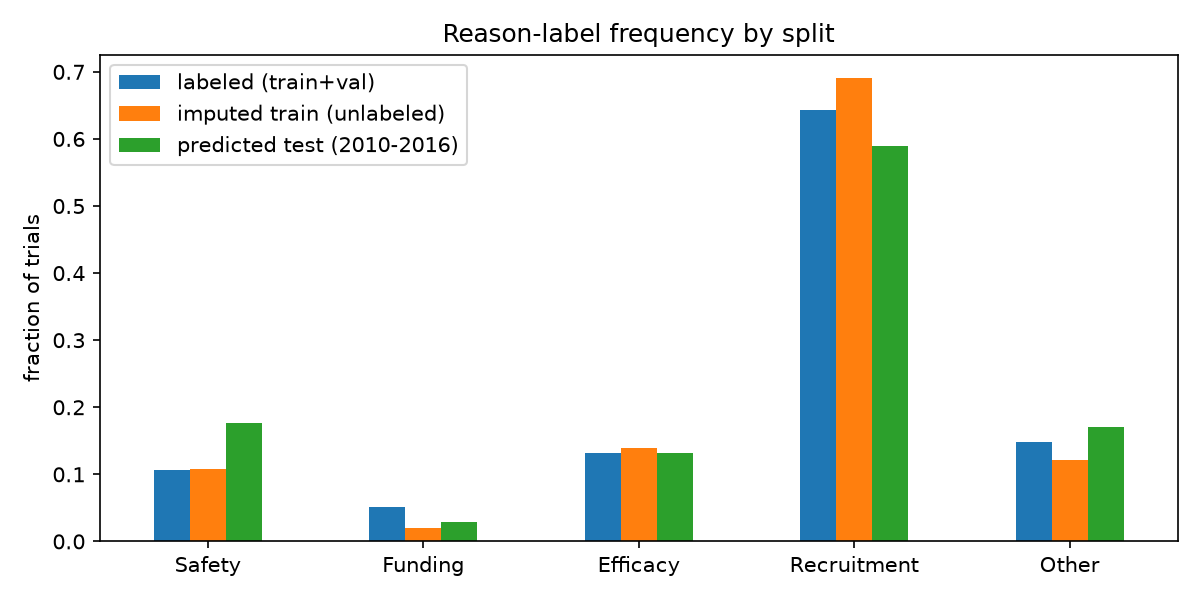
\includegraphics[width=0.95\linewidth]{part1_label_frequency.png}
\caption{Reason-label frequency across the labeled trials, the imputed unlabeled
training trials, and the predicted 2010--2016 test trials.}
\label{fig:p1freq}
\end{figure}

\subsection{Part 2}

Table~\ref{tab:p2val} reports per-phase validation metrics. Multinomial naive
Bayes separates classes about as well as logistic regression on ROC-AUC but is
wildly overconfident, so its log loss (2.646) is unusable for a log-loss
competition. The stack improves log loss and PR-AUC in every phase; adding
recency weights improves log loss further and recovers the F1 that the unweighted
stack gave up.

\begin{table}[t]
\centering\small
\setlength{\tabcolsep}{4pt}
\begin{tabular}{llcccc}
\toprule
Model & Phase & F1 & ROC-AUC & PR-AUC & log loss \\
\midrule
\multirow{4}{*}{MNB (per phase)}
 & I    & 0.737 & 0.717 & 0.733 & 2.684 \\
 & II   & 0.645 & 0.694 & 0.623 & 2.945 \\
 & III  & 0.796 & 0.699 & 0.783 & 2.308 \\
 & mean & 0.726 & 0.703 & 0.713 & 2.646 \\
\midrule
\multirow{4}{*}{Baseline LR (per phase)}
 & I    & 0.774 & 0.780 & 0.809 & 0.609 \\
 & II   & 0.631 & 0.729 & 0.711 & 0.610 \\
 & III  & 0.813 & 0.764 & 0.868 & 0.553 \\
 & mean & 0.739 & 0.758 & 0.796 & 0.591 \\
\midrule
\multirow{4}{*}{Improved: stacked}
 & I    & 0.730 & 0.772 & 0.816 & 0.570 \\
 & II   & 0.661 & 0.749 & 0.733 & 0.591 \\
 & III  & 0.817 & 0.787 & 0.883 & 0.516 \\
 & mean & 0.736 & 0.769 & 0.810 & 0.559 \\
\midrule
\multirow{4}{*}{\textbf{Final: $+$ recency ($\tau{=}3$)}}
 & I    & 0.793 & 0.793 & 0.828 & 0.557 \\
 & II   & 0.648 & 0.754 & 0.735 & 0.593 \\
 & III  & 0.824 & 0.787 & 0.881 & 0.518 \\
 & mean & \textbf{0.755} & \textbf{0.778} & \textbf{0.814} & \textbf{0.556} \\
\bottomrule
\end{tabular}
\caption{Part~2 validation metrics by phase. F1 uses a 0.5 threshold; ROC-AUC,
PR-AUC and log loss use predicted probabilities, with $\text{label}=1$ positive.}
\label{tab:p2val}
\end{table}

The time-based holdouts (Table~\ref{tab:p2holdout}) confirm the ordering under the
distribution shift that actually matters. Fitting on trials up to 2009 and scoring
2010--2013, the stack cuts log loss from 0.5879 to 0.5514 and recency weighting
takes it to 0.5475; on the harder 2012--2013 holdout the margin widens (0.5192
$\to$ 0.4657 $\to$ 0.4553).

\begin{table}[t]
\centering\small
\setlength{\tabcolsep}{4pt}
\begin{tabular}{llcccc}
\toprule
Holdout & Model & F1 & ROC-AUC & PR-AUC & log loss \\
\midrule
\multirow{4}{*}{fit $\leq$ 2009}
 & MNB       & 0.8083 & 0.6295 & 0.7301 & 2.4794 \\
 & Base.\ LR & 0.8051 & 0.6943 & 0.7847 & 0.5879 \\
 & Stacked   & 0.8090 & 0.7248 & 0.8183 & 0.5514 \\
 & $+$ rec.  & \textbf{0.8094} & \textbf{0.7311} & \textbf{0.8205} & \textbf{0.5475} \\
\midrule
\multirow{4}{*}{fit $\leq$ 2011}
 & MNB       & 0.8576 & 0.5970 & 0.7740 & 2.0120 \\
 & Base.\ LR & 0.8654 & 0.7042 & 0.8290 & 0.5192 \\
 & Stacked   & 0.8697 & 0.7539 & 0.8850 & 0.4657 \\
 & $+$ rec.  & \textbf{0.8758} & \textbf{0.7604} & \textbf{0.8865} & \textbf{0.4553} \\
\bottomrule
\end{tabular}
\caption{Part~2 time-based holdouts, mean over phases. The 2009 cut is evaluated
on 2010--2013 and the 2011 cut on 2012--2013. These mimic the later start years of
the test set and were used to select $\tau$.}
\label{tab:p2holdout}
\end{table}

On the Kaggle test set the final submission scores \textbf{0.58688} mean log loss
\TODO{confirm against leaderboard}, against 0.556 on validation---a gap we return
to in Section~\ref{sec:discussion}.

\subsection{Error analysis across reason categories}

Table~\ref{tab:p2errors} and Figure~\ref{fig:p2err} break the failed validation
trials down by phase and stopping reason. Two patterns are robust. First, error
rates are much higher in Phase~III (0.57--1.00 for the baseline) than in Phase~II
(0.00--0.38), despite Phase~III having more training data. Second, the largest and
therefore most trustworthy groups---Phase~II Recruitment ($n{=}87$) and the three
no-recorded-reason groups ($n{=}28/144/82$)---all improve monotonically from
baseline to stack to recency-weighted stack; the Phase~I no-reason group falls
from 0.643 to 0.321.

\begin{figure*}[t]
\centering
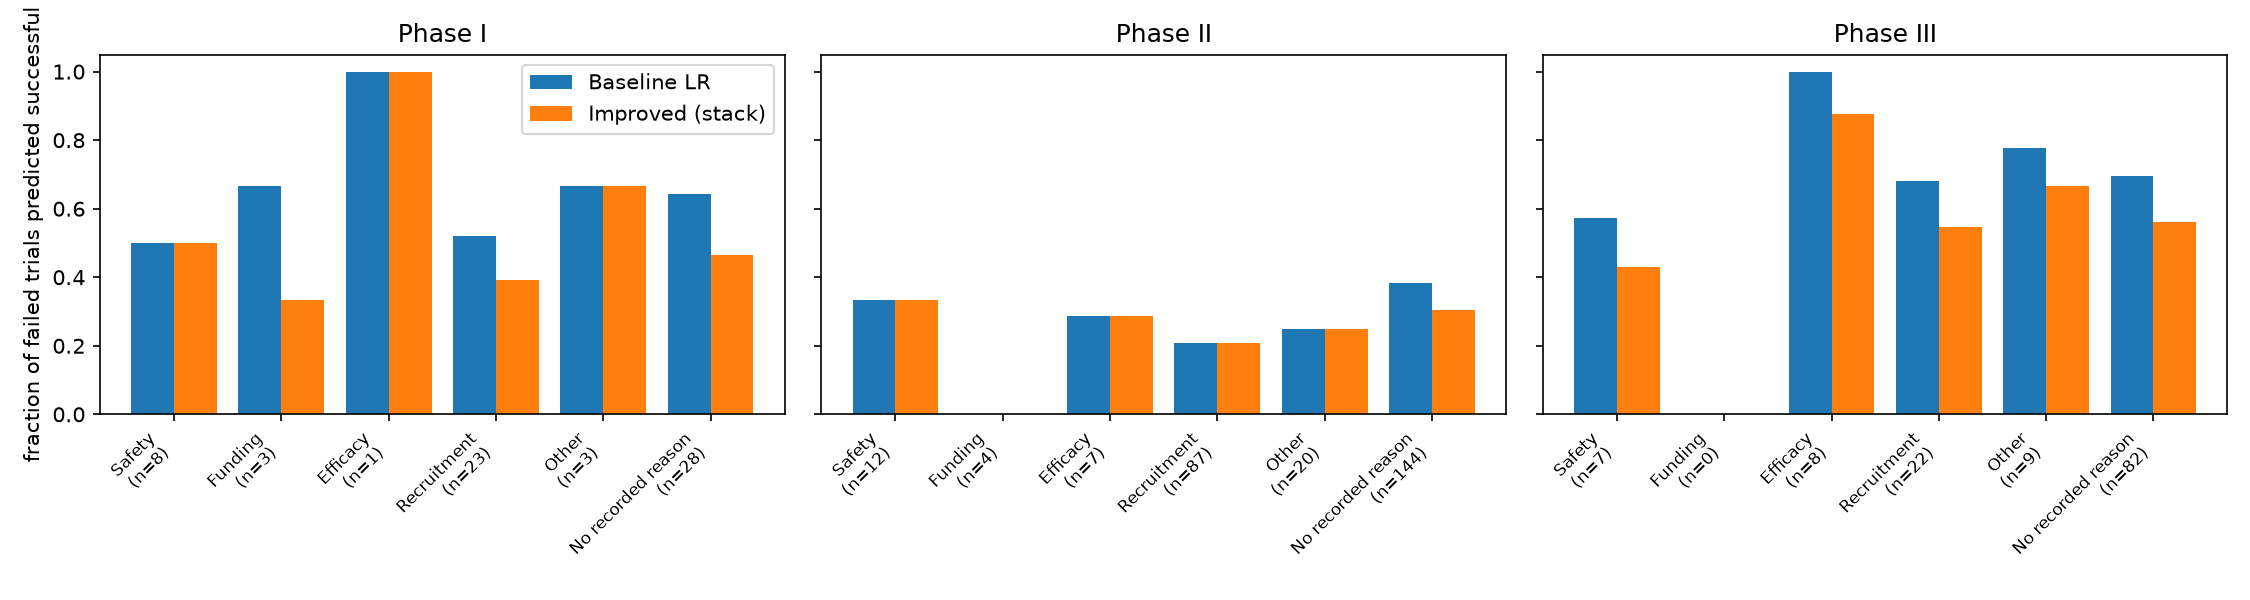
\includegraphics[width=\textwidth]{part2_error_by_reason.png}
\caption{Fraction of failed validation trials incorrectly predicted successful,
by phase and stopping reason, for the criteria-only baseline and the stacked
ensemble. Group sizes are given in the tick labels.}
\label{fig:p2err}
\end{figure*}

\begin{table*}[t]
\centering\small
\begin{tabular}{llccccccc}
\toprule
& & \multicolumn{3}{c}{Group composition} & & \multicolumn{3}{c}{Fraction predicted successful} \\
\cmidrule(lr){3-5}\cmidrule(lr){7-9}
Phase & Reason & $n$ trials & $n$ true & $n$ predicted & & Baseline LR & Improved & Final \\
\midrule
I & Safety             &  8 &  1 &  7 & &  0.500 & 0.500 & 0.375 \\
I & Funding            &  3 &  1 &  2 & &  0.667 & 0.333 & 0.000 \\
I & Efficacy           &  1 &  0 &  1 & &  1.000 & 1.000 & 0.000 \\
I & Recruitment        & 23 &  2 & 21 & &  0.522 & 0.391 & 0.174 \\
I & Other              &  3 &  0 &  3 & &  0.667 & 0.667 & 0.667 \\
I & No recorded reason & 28 &  0 &  0 & &  0.643 & 0.464 & 0.321 \\
\midrule
II & Safety             &  12 &  1 & 11 & & 0.333 & 0.333 & 0.250 \\
II & Funding            &   4 &  1 &  3 & & 0.000 & 0.000 & 0.000 \\
II & Efficacy           &   7 &  0 &  7 & & 0.286 & 0.286 & 0.286 \\
II & Recruitment        &  87 & 12 & 75 & & 0.207 & 0.207 & 0.149 \\
II & Other              &  20 &  3 & 17 & & 0.250 & 0.250 & 0.250 \\
II & No recorded reason & 144 &  0 &  0 & & 0.382 & 0.306 & 0.250 \\
\midrule
III & Safety             &  7 & 1 &  6 & & 0.571 & 0.429 & 0.429 \\
III & Funding            &  0 & 0 &  0 & & ---   & ---   & ---   \\
III & Efficacy           &  8 & 0 &  8 & & 1.000 & 0.875 & 1.000 \\
III & Recruitment        & 22 & 5 & 17 & & 0.682 & 0.545 & 0.455 \\
III & Other              &  9 & 2 &  7 & & 0.778 & 0.667 & 0.556 \\
III & No recorded reason & 82 & 0 &  0 & & 0.695 & 0.561 & 0.585 \\
\bottomrule
\end{tabular}
\caption{Error rates on the 452 failed validation trials, by phase and stopping
reason. ``$n$ true'' counts trials whose reason labels are ground truth from
Part~1; ``$n$ predicted'' counts trials whose reason labels are Part~1 model
predictions. A trial with several reasons appears in each of its reason rows, so
columns do not sum to the phase total.}
\label{tab:p2errors}
\end{table*}

\section{Discussion}
\label{sec:discussion}

\paragraph{Clustering is a poor labeler but a useful prior.}
Used directly, the 30-component mixture is the worst model in
Table~\ref{tab:p1models} (0.780 sample-F1, 0.570 macro-F1). Inspecting the
components explains why: they overwhelmingly separate Recruitment from
everything else, and additional components mostly subdivide Recruitment further
rather than isolating Safety or Efficacy. Since the embeddings do carry that
signal---a purely supervised model reaches Safety F1 0.947---the failure is the
clustering objective, not the features. Unsupervised structure in this space
tracks the dominant topic, and with Recruitment on 64\% of trials the dominant
topic is Recruitment. What does work is demoting the mixture from decision-maker
to prior: as a 0.2-weighted term inside the pseudo-labeling step it raises
cross-validated macro-F1 from 0.805 to 0.814 (and validation sample-F1 from 0.889
to 0.893) over identical self-training without it. The mixture's contribution is
to regularize which unlabeled trials get promoted, not to name their reasons.

\paragraph{Why the extra features fail.}
This is the ablation's most informative result. The reason embeddings are a
compressed encoding of the very stopping-reason text the labels were derived
from, so they are close to a sufficient statistic for the target. Criteria,
disease and drug fields describe \emph{what the trial was}, not \emph{why it
stopped}---a trial can be halted for funding reasons regardless of its indication.
Appending them adds 20--50 parameters per block to a model fit on 157 labeled
trials, so the variance cost arrives immediately while the bias reduction never
does: criteria TF-IDF drops validation sample-F1 from 0.893 to 0.876. The Morgan
fingerprints are the clearest null result, moving cross-validated macro-F1 by
$+0.001$---within repeat-to-repeat noise---which is unsurprising given that 44\%
of trials have no matched drug and receive an all-zero block. \texttt{start\_year}
fails for a more interesting reason: it is genuinely predictive in-sample, because
the labeled trials are deliberately the earliest ones, but the test trials are the
latest, so the model would be extrapolating a year effect fit entirely outside the
test range. Including everything is actively harmful here, not merely redundant.

\paragraph{Rare labels dominate macro-F1.}
Recruitment appears on 64\% of trials and Funding on 5\%. Funding F1 (0.400) and
Other F1 (0.500) rest on 4 and 10 positive validation trials respectively, so a
single trial moves macro-F1 by several points. This is why the validation macro-F1
column in Table~\ref{tab:p1models} is non-monotone with the CV column, and why we
selected on the latter: the final model has slightly lower validation macro-F1
than the balanced LR + $k$NN blend (0.714 vs.\ 0.724) but the best CV macro-F1
(0.814 vs.\ 0.800), and the 235-trial CV estimate is the more reliable of the two.

\paragraph{What the stack buys in Part 2.}
The fitted meta-model weights are informative: criteria LR 0.62, criteria $k$NN
0.55, drug-name LR 0.41, metadata 0.16, with disease (0.06) and ICD (0.03) nearly
ignored and drug-knowledge slightly negative ($-0.11$). The drug-knowledge block
is not useless in isolation---it is redundant once drug names are present, since
targets and pathways are a deterministic function of the matched drug, and the
meta-model subtracts it as a partial correction. The $k$NN's large weight shows
the stack is exploiting near-duplicate trials that the linear criteria model
cannot represent. Pooling phases matters most for Phase~I, which has only 1,012
training rows and gains the most from the shared representation.

\paragraph{The F1 / log-loss trade-off.}
The unweighted stack \emph{lowers} mean validation F1 from 0.739 to 0.736 while
improving log loss (0.591 $\to$ 0.559) and PR-AUC (0.796 $\to$ 0.810). This is not
a regression: F1 at a fixed 0.5 threshold is a statement about calibration near
that threshold, and the stack's meta-model shifts probabilities toward the base
rate, pushing borderline positives below 0.5. Ranking quality, which is what
ROC-AUC and PR-AUC measure, improves in every phase. Recency weighting then raises
the probabilities again and lifts F1 to 0.755, better than either predecessor.
Since the competition metric is log loss, we optimized for calibration and treat
the F1 recovery as a bonus; a project scored on F1 would instead have tuned the
threshold per phase.

\paragraph{Where the errors live.}
The strongest signal in Table~\ref{tab:p2errors} is that failure is hardest to
detect in Phase~III and among trials with no recorded stopping reason. Both follow
from the same cause: these are trials that ran to completion and missed their
endpoint, so nothing in the eligibility text, indication or drug marks them as
different from a successful trial---and Phase~III has a 0.65 success base rate
pulling predictions upward. By contrast, trials stopped for Recruitment or Funding
are administrative failures, and the stack catches them better (Phase~II
Recruitment 0.207 $\to$ 0.149) partly because small, slow-recruiting trials leave
traces in criteria length and drug-count metadata. The improvement is largest
exactly where the baseline was worst: Phase~I no-reason 0.643 $\to$ 0.321,
Phase~III no-reason 0.695 $\to$ 0.585.

\paragraph{How much of the error table to believe.}
Two caveats temper this. Category sizes are small---Safety, Funding, Efficacy and
Other have fewer than 25 failed trials in every phase, and Phase~III Efficacy has
8, so its apparent 1.000 $\to$ 0.875 $\to$ 1.000 trajectory is one trial moving.
Phase~III Funding has no trials at all. More subtly, 171 of the 198 matched reason
labels are Part~1 \emph{predictions} rather than ground truth, and the Part~1
model has roughly 10\% sample-F1 error. Those errors are not random: because the
Part~1 model over-predicts the majority reason, trials are more likely to be
misfiled \emph{into} Recruitment than out of it, which biases the Recruitment row
toward the population average and makes the rare-reason rows noisier than their
sample sizes alone suggest. Only the Phase~II Recruitment row and the three
no-reason rows (whose membership is determined by a join, not a prediction, and so
is error-free) support confident conclusions.

\paragraph{The validation-to-test gap.}
Mean log loss rises from 0.556 on validation to 0.58688 on Kaggle. The cause is
temporal: validation trials started up to 2013 and were split at random from the
training trials, while test trials started 2013--2022, later than every training
row, and the success rate climbs from 0.38 in 2000 to 0.81 in 2013. A model fit on
the pooled base rate is therefore systematically under-confident on test. Recency
weighting is our response and was the single largest holdout gain we found
(0.5514 $\to$ 0.5475 fitting to 2009; 0.4657 $\to$ 0.4553 fitting to 2011); it
redistributes mean test predictions per phase rather than inflating them
uniformly---Phase~III rises from 0.711 to 0.738 while Phase~I falls from 0.617 to
0.598 and Phase~II from 0.565 to 0.557---because recent Phase~III trials succeeded
far more often than recent early-phase ones. The residual gap reflects what we deliberately did not model. We
built an alternative submission that lets the meta-model learn an explicit
Phase~III year trend (Phase~III success rises 0.71 in 2009 to 0.96 in 2013), which
pushes mean Phase~III test predictions to 0.788; on the holdouts it gains only
about 0.001 log loss, and it extrapolates a trend fit on four years out to 2022,
so we kept it as a recorded alternative rather than the submission. A per-phase
trend for all phases was rejected outright: it fits flat or negative Phase~I/II
slopes and would drive those predictions below the training base rate. Beyond the
year effect, the test trials differ in disease and drug mix, and no amount of
reweighting on pre-2014 data can calibrate for that.


{
    \small
    \bibliographystyle{ieeenat_fullname}
    \bibliography{main}
}

\end{document}
